% =====================================================================
%  BLG 345E Logic and Computability - Term Project Phase 1 Report
%  Compile from the report/ folder:   latexmk -pdf report.tex
%  (or upload the whole report/ folder to Overleaf, main file report.tex)
% =====================================================================
\documentclass[11pt,a4paper]{article}
\PassOptionsToPackage{obeyspaces,spaces}{url}


\newcommand{\teamno}{02}
\newcommand{\members}{%
  Eylül Ebrar Gülbeyaz      & 820230304 & \code{my_checker}, test suite, Peterson, report \\
  Emirhan Ulu        &  820230317 & Dining Philosophers, report \\
  Turgut Emre Sürenkök       & 820230322 & Alternating Bit Protocol , report\\
  Eren Süslü       & 820230323 & Railway Crossing Controller, report \\
  Oğuz Ünlüoğlu      & 820260713 & Three-Floor Elevator Controller, report \\
}
% ---------------------------------------------------------------------

\usepackage[T1]{fontenc}
\usepackage[utf8]{inputenc}
\usepackage{lmodern}
\usepackage{microtype}
\usepackage[margin=2.3cm]{geometry}
\usepackage{graphicx}
\usepackage{booktabs}
\usepackage{tabularx}
\usepackage{longtable}
\usepackage{array}
\usepackage{xcolor}
\usepackage{listings}
\usepackage{enumitem}
\usepackage{float}
\usepackage{caption}
\usepackage{amsmath,amssymb}
\usepackage{fancyhdr}
\usepackage{tikz}
\usetikzlibrary{positioning,arrows.meta}
\usepackage[hidelinks]{hyperref}

% --- helpers ---------------------------------------------------------
\usepackage{url}
\DeclareUrlCommand\codeurl{\urlstyle{tt}}
\DeclareRobustCommand{\code}{\codeurl}
\makeatletter
\g@addto@macro\UrlBreaks{\do\_\do\=\do\(\do\>}
\g@addto@macro\UrlSpecials{\do\'{\mbox{\textquotesingle}}}
\makeatother
\Urlmuskip=0mu plus 1mu
\newcommand{\todo}[1]{\textcolor{red}{\textbf{[#1]}}}
\newcolumntype{L}{>{\raggedright\arraybackslash}X}
\newcolumntype{C}{>{\centering\arraybackslash}X}
\setlist{itemsep=2pt,topsep=4pt}
\captionsetup{font=small,labelfont=bf}

\definecolor{codebg}{HTML}{F6F8FA}
\definecolor{codeframe}{HTML}{D0D7DE}
\definecolor{kw}{HTML}{0B5CAD}
\definecolor{cm}{HTML}{6A737D}
\definecolor{hlred}{HTML}{F8C9C4}
\definecolor{hlgreen}{HTML}{CDEBC6}
\definecolor{hlblue}{HTML}{CFE0F5}
\lstset{
  basicstyle=\ttfamily\footnotesize,
  backgroundcolor=\color{codebg},
  frame=single, rulecolor=\color{codeframe},
  framesep=4pt, xleftmargin=6pt, xrightmargin=6pt,
  breaklines=true, breakatwhitespace=false,
  columns=fullflexible, keepspaces=true,
  showstringspaces=false, upquote=true,
  literate={∅}{{$\emptyset$}}1,
  aboveskip=6pt, belowskip=6pt,
}
\lstdefinestyle{py}{language=Python, keywordstyle=\color{kw}\bfseries,
  commentstyle=\color{cm}\itshape}
\lstdefinelanguage{smv}{
  morekeywords={MODULE,main,VAR,IVAR,ASSIGN,DEFINE,INIT,TRANS,init,next,case,esac,
    TRUE,FALSE,boolean,LTLSPEC,INVARSPEC,in,G,F,X},
  sensitive=true, morecomment=[l]{--}}
\lstdefinestyle{smv}{language=smv, keywordstyle=\color{kw}\bfseries,
  commentstyle=\color{cm}\itshape}
\newcommand{\console}[2]{\par\noindent\begin{minipage}{\linewidth}\lstinputlisting[caption={#2},captionpos=b]{#1}\end{minipage}\par\smallskip}

\pagestyle{fancy}
\fancyhf{}
\lhead{\small BLG 345E -- Project Phase 1}
\rhead{\small Team \teamno}
\cfoot{\small\thepage}
\setlength{\headheight}{14pt}

\begin{document}

% =====================================================================
\begin{titlepage}
\centering
{\large Istanbul Technical University\\
Faculty of Computer and Informatics Engineering\\
Department of Computer Engineering\par}
\vspace{2.2cm}
{\Large BLG 345E -- Logic and Computability\par}
\vspace{0.6cm}
{\huge\bfseries Term Project -- Phase 1\par}
\vspace{0.3cm}
{\Large Structural Modeling, Parsing and Oracle Validation\par}
\vspace{1.6cm}
{\Large Team \teamno\par}
\vspace{0.8cm}
\begin{tabular}{lll}
\toprule
\textbf{Name} & \textbf{Student ID} & \textbf{Main responsibility}\\
\midrule
\members
\bottomrule
\end{tabular}
\vfill
{\large Instructor: Asst.\ Prof.\ Mehmet Tahir Sandıkkaya\\[2pt]
Teaching Assistants: Res.\ Assist.\ Ali Esad Uğur, Res.\ Assist.\ Nurkan Fatih Altunel\par}
\vspace{0.8cm}
{\large Fall 2026\par}
\end{titlepage}

\tableofcontents
\newpage

% =====================================================================
\section*{Overview}
\addcontentsline{toc}{section}{Overview}

In this phase we prepared the groundwork for our explicit-state LTL model
checker, following the project assignment~\cite{assignment}. We modeled each
of the five systems twice. The first version is a JSON file in the common
schema that lists every state and transition explicitly. The second is a
NuSMV model that describes the same system through variables and update rules.
Both describe the same Kripke structure $M=(S,S_0,R,L)$ from the lectures on
model checking~\cite{slides}. Our tool \code{my_checker} reads a JSON model,
validates it, stores it as an adjacency-list graph and runs a breadth-first
search to find the reachable states. We then used NuSMV as a reference and
checked that it finds the same reachable states as our tool.

\begin{table}[H]
\centering\small
\caption{Summary of the five models. ``Domain'' is the product of the SMV state-variable domains; ``Reachable'' is reported identically by \code{my_checker} and NuSMV.}
\label{tab:summary}
\resizebox{\textwidth}{!}{%
\begin{tabular}{lllrrrr}
\toprule
\textbf{System} & \textbf{Semantics} & \textbf{State variables} & \textbf{Domain} & \textbf{Reachable} & \textbf{Transitions} & \textbf{Self-loops}\\
\midrule
Dining Philosophers & interleaving & \code{p0, p1, p2}                  & 27  & 14 & 28 & 1\\
Peterson            & interleaving & \code{pc0, pc1, turn}              & 32  & 20 & 40 & 6\\
Alternating Bit     & channel input & \code{s_bit, r_bit, phase}        & 28  & 22 & 32 & 0\\
Railway Crossing    & synchronous  & \code{train, gate, ctrl}           & 48  & 29 & 80 & 14\\
Elevator            & controller step & \code{pos, dir, door, req, stalled} & 480 & 43 & 58 & 9\\
\bottomrule
\end{tabular}}
\end{table}

All deliverables are in the submitted folder:

\begin{center}\small
\begin{tabularx}{\textwidth}{lL}
\toprule
\textbf{Path} & \textbf{Content}\\
\midrule
\code{my_checker} & executable entry point (POSIX shell script that launches \code{src/checker.py} with Python~3)\\
\code{src/checker.py} & parser, schema/semantic validation, graph data structure, BFS reachability\\
\code{models/} & the ten required files \code{<system>.json} and \code{<system>.smv}\\
\code{scripts/gen_<system>.py} & generators that produce each JSON model by explicit state exploration\\
\code{scripts/draw_model.py}, \code{report_figures.py} & Graphviz state-diagram renderers\\
\code{scripts/run_all.sh}, \code{compare_nusmv.py} & reproduce every console output in this report and compare state sets with NuSMV\\
\code{tests/} & light-switch example and the valid/invalid parser test models\\
\code{report/} & this report, figures and the recorded console outputs\\
\bottomrule
\end{tabularx}
\end{center}

All console outputs shown in this report were produced by running
\code{sh scripts/run_all.sh} from the project root, so they can be reproduced
at any time. We used Python~3 with only its standard library, Graphviz for the
diagrams, and NuSMV~2.7.1.

% =====================================================================
\section{Modeling Methodology}
\label{sec:method}

\subsection{Common conventions}

We followed the same approach for all five systems so that the two
representations stay easy to compare.

For each system we first chose a small set of state variables, usually one per
component plus any shared variable. These are exactly the \code{VAR} variables
of the SMV model. A JSON state is one assignment of values to these variables,
and we build its identifier from those values, for example
\code{InCrossing__Lowering__ClosingRequested}. This way every JSON state
corresponds to exactly one SMV state and the other way around.

Some choices in the systems come from the environment rather than from the
system itself: which process runs next in Peterson, what the channel does in
ABP, and the floor calls and emergency button in the elevator. We declared
these as \code{IVAR} in SMV. NuSMV does not count input variables as part of
the state, and they do not appear in our JSON states either. Their only effect
is that a state can have several outgoing transitions.

The atomic propositions are not stored separately. In SMV each one is a
\code{DEFINE} over the state variables, and the JSON generators compute the
labels with the same conditions. We used only the proposition names given in
the assignment.

We did not write the JSON files by hand. Each \code{scripts/gen_<system>.py}
encodes the rules of its system, starts from the initial state and explores
the state space with BFS. As a result, every JSON model contains only
reachable states and reports 0 unreachable states. The \code{.smv} files were
written by hand and separately from the generators, and we did not translate
one format into the other. When the two agree, it is therefore a real check
and not a copy.

Finally, following Section~4 of the assignment, a configuration from which
nothing can happen (a deadlock or a terminal state) gets a self-loop. We used
self-loops in the same way for busy waiting: a process that tries to proceed
but is blocked takes a step that leaves the state unchanged.

\subsection{Problem 1 -- Dining Philosophers}

Three philosophers $P_0,P_1,P_2$ share three forks. Fork $f_i$ is the left
fork of $P_i$ and the right fork of $P_{(i+2)\bmod 3}$, so $P_i$ eats with
$f_i$ on its left and $f_{(i+1)\bmod 3}$ on its right.

Each philosopher is \code{Thinking} (T), \code{HoldingLeft} (L) or
\code{Eating} (E), and all of them start in T. We decided not to keep the
forks as separate variables. A fork is in use exactly when its left owner is
in L or E, or its right owner is in E, so the state of the forks can always be
read from the philosophers. In other words, $f_i$ is free iff
$P_i\notin\{L,E\}$ and $P_{(i+2)\bmod 3}\neq E$. Separate fork variables would
only repeat this information.

The model uses interleaving: in each transition one philosopher does one
thing. A thinking philosopher picks up its left fork if it is free (T$\to$L),
a philosopher holding its left fork picks up the right one if it is free
(L$\to$E), and an eating philosopher puts both forks down (E$\to$T).

When all three philosophers hold their left forks (LLL), each one waits for a
fork that its neighbor holds, and nobody can move. This is the only state in
which no action is possible. We labeled it \code{deadlock} and gave it a
self-loop.

\subsection{Problem 2 -- Peterson's Mutual Exclusion}

Each process $P_i$ runs the reference algorithm from the assignment. We gave
its program counter one value for each atomic statement:

\begin{center}\small
\begin{tabular}{lll}
\toprule
\textbf{\code{pc_i}} & \textbf{Position in the algorithm} & \textbf{Effect of the next step}\\
\midrule
\code{idle}     & remainder section             & \code{flag[i] = true}\\
\code{flag_set} & flag raised, turn not yet set & \code{turn = j}\\
\code{waiting}  & in the \code{while} loop      & enter CS if \code{!(flag[j] && turn == j)}, otherwise stay\\
\code{critical} & critical section              & \code{flag[i] = false}, back to \code{idle}\\
\bottomrule
\end{tabular}
\end{center}

Like the forks in the previous problem, the flags are not stored separately.
\code{flag[i]} is raised by the step that leaves \code{idle} and lowered by the
step that returns to it, so it is true exactly when \code{pc_i} $\neq$
\code{idle}.

To model interleaving we added an input \code{proc} $\in\{0,1\}$ that picks
which process takes the next step. Every state therefore has one successor for
each process, at most two in total. If the chosen process is in
\code{waiting} and the loop condition still holds, it has to keep waiting and
the state does not change. These busy-wait steps are the 6 self-loops of the
model. The initial state is (\code{idle}, \code{idle}, turn~=~0), which means
both flags are false and turn is 0, as the assignment requires.

\subsection{Problem 3 -- Alternating Bit Protocol}

Since the sender never has more than one unacknowledged packet and the
channel does not reorder, we only follow the life of that one packet. The
state consists of the sender bit \code{s_bit}, the receiver's expected bit
\code{r_bit} (both 0 at the start) and a \code{phase} variable with 7 values
that says where the packet or its ACK currently is. What the channel does in
each step is an input, \code{channel} $\in\{$\code{deliver}, \code{lose},
\code{corrupt}$\}$.

A transmission starts with \code{ready} $\to$ \code{data_sent}, and the sender
does not send anything new until this packet is acknowledged or times out.
From \code{data_sent} there are three possibilities. If the packet is lost we
move to \code{pkt_lost}, where \code{packet_lost} holds. If it is corrupted,
the receiver notices this with its abstract error check, throws the packet
away and leaves \code{r_bit} as it is; we move to \code{pkt_corrupted}, where
\code{bit_error} holds. Both of these continue to \code{timeout}, and from
\code{timeout} the sender sends the same packet again with the same
\code{s_bit}. This cycle is the timeout loop asked for in the assignment.

If the packet arrives and its bit matches \code{r_bit}, the receiver accepts
it, flips \code{r_bit} and sends an ACK (\code{ack_sent}). If the bits do not
match, the packet is a duplicate of one that was already accepted. The
receiver does not accept it a second time, but it sends the ACK again, since
the earlier ACK was probably lost.

From \code{ack_sent}, a delivered ACK takes us to \code{ack_rcvd}, where
\code{ack_received} holds; the sender then flips \code{s_bit} and goes back to
\code{ready}. Any other channel outcome means the ACK did not arrive and we go
to \code{timeout}. We treated a corrupted ACK the same as a lost one, because
the sender cannot use it either way. We also did not model the timer itself:
after a loss or a rejected packet, the timeout simply happens in the next step
and forces the retransmission.

\subsection{Problem 4 -- Railway Crossing Controller}

The model is the synchronous product of three state machines: Train (Far,
Approaching, InCrossing, Passed), Gate (Open, Lowering, Closed, Raising) and
Controller (Idle, ClosingRequested, OpeningRequested). It starts in (Far,
Open, Idle). In every step all three components update at the same time. Each
one either makes one allowed move or stays where it is, and all of them decide
based on the values from before the step.

The train is not controlled by anything. In each step it either stays or
moves one position along Far $\to$ Approaching $\to$ InCrossing $\to$ Passed
$\to$ Far. Because the gate never blocks it, the train can enter the crossing
before the gate has closed, which is the fast-train scenario described in the
assignment.

We made the controller deterministic. It switches from Idle to
ClosingRequested when it sees the train Approaching (or already InCrossing),
from ClosingRequested to OpeningRequested when it sees the train Passed, and
from OpeningRequested back to Idle once the gate is Open again. The gate
reacts to these commands. On a closing request it goes from Open to Lowering,
stays in Lowering for at least one step (possibly more) and then reaches
Closed. On an opening request it goes from Closed to Raising, and after some
time from Raising to Open.

One consequence of this design is that the controller only reacts to a new
train after the previous opening cycle is complete. If a train comes back
while the gate is still raising, we get additional unsafe states. We kept this
behavior on purpose, because it is a real weakness of the controller as
specified. Since every component can always choose to stay, we did not need
any artificial self-loops. The 14 self-loops in the model are steps where all
three components stay.

\subsection{Problem 5 -- Three-Floor Elevator Controller}

The state of the elevator is (\code{pos}, \code{dir}, \code{door},
\code{req}, \code{stalled}), and one transition is one controller step. In
each step the environment can press a floor button (\code{call} $\in\{$none,
F1, F2, F3$\}$) and the \code{emergency} button. Apart from these inputs the
controller always does the same thing in the same situation.

The position \code{pos} takes the values F1, F1\_2, F2, F2\_3 and F3, so the
positions between floors are explicit, as the assignment asks. The cabin moves
one position per step and therefore only ever travels between adjacent floors.
The elevator handles one request at a time. A call is accepted only when the
cabin is idle (stationary, doors closed, no request), and the request is
cleared when the doors have closed again. A call for the floor the cabin is
already on is also accepted and simply starts the door cycle.

The cabin can only start moving when the doors are completely closed, and the
doors stay closed while it moves. When it reaches the requested floor, it
first stops (\code{dir} becomes Stationary), and only in the next step do the
doors start to open. The doors then go through Closed $\to$ Opening $\to$ Open
$\to$ Closing $\to$ Closed, one phase per step, so they always close again
after opening. If the request is for another floor, the cabin passes Floor~2
without stopping.

We allowed the emergency stop only while the cabin is moving at an
intermediate position, because the assignment requires the stalled state to
be between floors. After an emergency stop the cabin is Stationary, its doors
are Closed and locked, and \code{stalled} is true. A stalled state is terminal
and has only a self-loop. We kept the pending request in the stalled state, so
it still shows where the cabin was going. An idle cabin with no new call also
has a self-loop. Together these give the 9 self-loops of the model: 3 idle
states and 6 stalled states.

% =====================================================================
\section{State-Space Representations}
\label{sec:statespace}

In the diagrams below, the initial state has a bold border and an arrow
pointing to it. Each box shows the JSON identifier of the state and, in
braces, the propositions that are true there ($\emptyset$ if none). We used
colors to make the interesting states easier to find:
red for dangerous or terminal states,
green for states where something useful happens, and
blue for states where the elevator is moving. The diagrams
are generated from the JSON models with Graphviz
(\code{scripts/draw_model.py}). In the railway diagram the long state names
are split onto several lines at each \code{__} so that the boxes stay narrow.
The figures are vector graphics, so they can be zoomed in the PDF.

% ---------------------------------------------------------------------
\subsection{Dining Philosophers}

\begin{center}\small
\begin{tabularx}{\textwidth}{lll L}
\toprule
\textbf{Kind} & \textbf{Name} & \textbf{Domain / definition} & \textbf{Meaning}\\
\midrule
variable & \code{p0}, \code{p1}, \code{p2} & \{thinking, holding\_left, eating\} & local state of each philosopher\\
proposition & \code{Pi_eating} & \code{pi = eating} & philosopher $i$ is eating\\
proposition & \code{deadlock} & all three \code{holding_left} & circular wait\\
\bottomrule
\end{tabularx}
\end{center}

\textbf{State IDs.} \code{s_XYZ} with $X,Y,Z\in\{T,L,E\}$ the states of
$P_0,P_1,P_2$; for example \code{s_TLE}.

\textbf{Size.} There are $3^3=27$ possible combinations, of which 14 are
reachable, with 28 transitions. The 13 combinations that never occur are the
ones where the same fork would be held by two philosophers at once. In 7 of
them two philosophers are eating at the same time (with three philosophers,
any two are neighbors). In the other 6, one philosopher is eating while a
neighbor holds the shared fork as its left fork. For example, in \code{ELT}
$P_0$ would be eating with $f_0$ and $f_1$ while $P_1$ also holds $f_1$. Every
eating state has two successors: the eating philosopher puts the forks down,
or a neighbor that can still take a fork takes it. The only self-loop belongs
to the \code{deadlock} state \code{s_LLL}.

\begin{figure}[H]
\centering
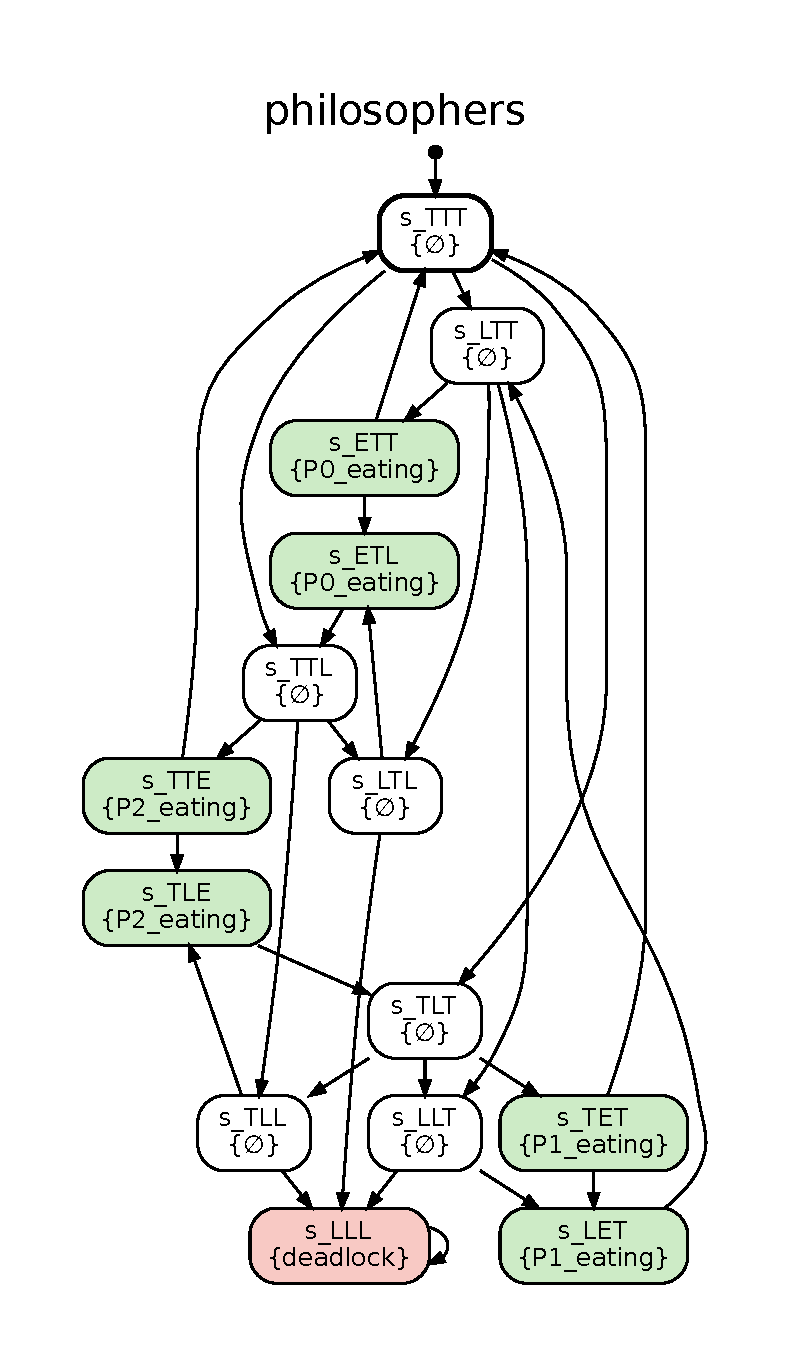
\includegraphics[height=0.62\textheight]{figures/philosophers.pdf}
\caption{Dining Philosophers: 14 states, 28 transitions. Green: some
philosopher eats. Red: deadlock (\code{s_LLL}, self-loop).}
\label{fig:phil}
\end{figure}

% ---------------------------------------------------------------------
\subsection{Peterson's Mutual Exclusion}

\begin{center}\small
\begin{tabularx}{\textwidth}{lll L}
\toprule
\textbf{Kind} & \textbf{Name} & \textbf{Domain / definition} & \textbf{Meaning}\\
\midrule
variable & \code{pc0}, \code{pc1} & \{idle, flag\_set, waiting, critical\} & program counters\\
variable & \code{turn} & \{0, 1\} & shared turn variable\\
input & \code{proc} & \{0, 1\} & process executing this step\\
proposition & \code{P0_in_CS}, \code{P1_in_CS} & \code{pci = critical} & process $i$ in its critical section\\
proposition & \code{flag0}, \code{flag1} & \code{pci != idle} & interest flag of process $i$\\
proposition & \code{turn_is_1} & \code{turn = 1} & priority given to $P_1$\\
\bottomrule
\end{tabularx}
\end{center}

\textbf{State IDs.} \code{<pc0>__<pc1>__t<turn>}, for example
\code{waiting__flag_set__t1}.

\textbf{Size.} There are $4\cdot 4\cdot 2=32$ possible combinations and 20
of them are reachable. Each reachable state has two outgoing transitions, one
for each process, which gives 40 transitions. The states where both processes
want to enter the critical section are included, for example
\code{waiting__waiting__t0} and \code{waiting__waiting__t1}. There is no
reachable state where \code{P0_in_CS} and \code{P1_in_CS} are both true.

\begin{figure}[H]
\centering
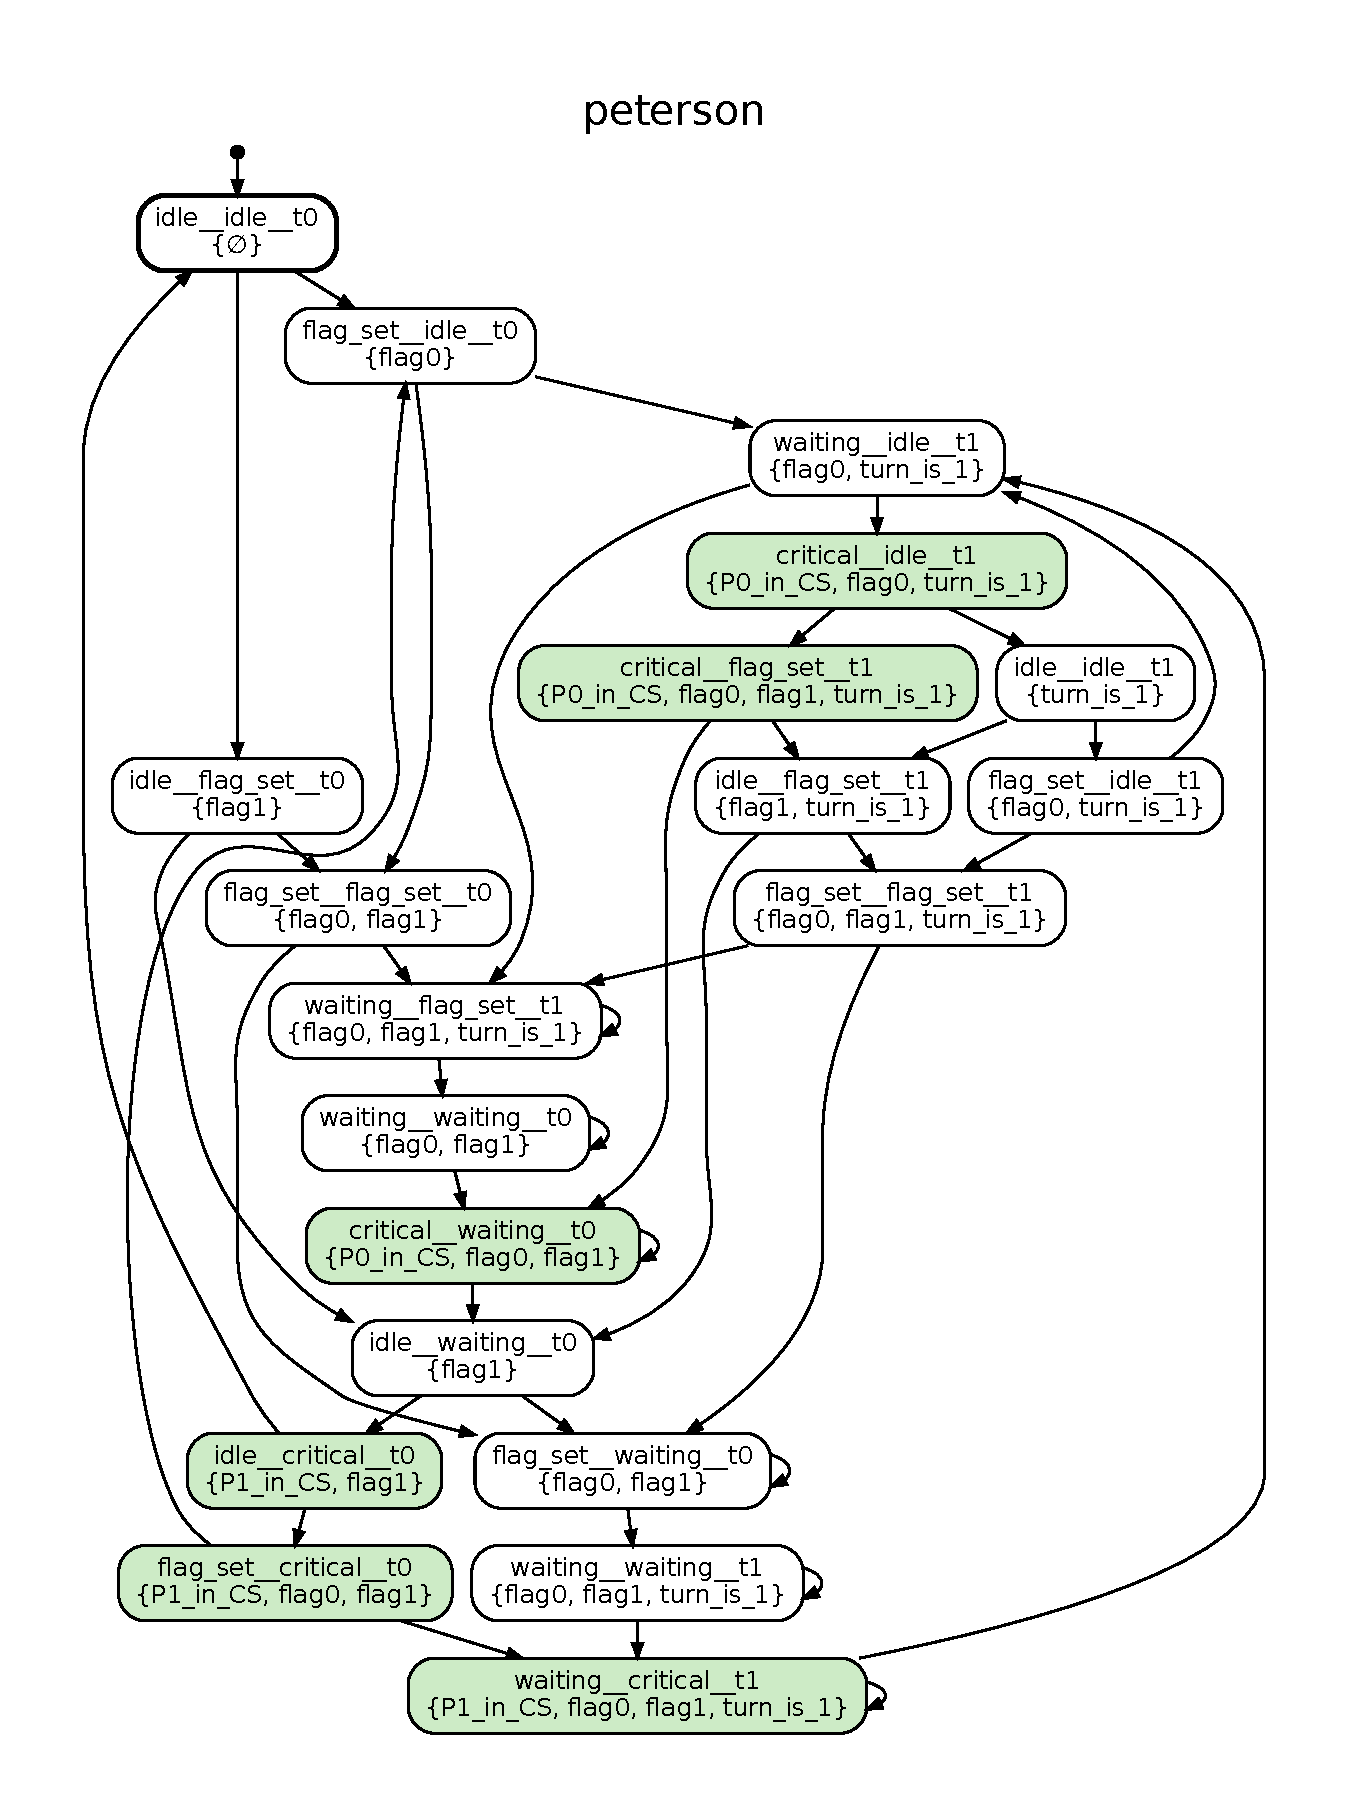
\includegraphics[width=\textwidth,height=0.85\textheight,keepaspectratio]{figures/peterson.pdf}
\caption{Peterson's algorithm: 20 states, 40 transitions. Green: one process
is in its critical section. The self-loops are blocked busy-wait steps.}
\label{fig:peterson}
\end{figure}

% ---------------------------------------------------------------------
\subsection{Alternating Bit Protocol}

\begin{center}\small
\begin{tabularx}{\textwidth}{lll L}
\toprule
\textbf{Kind} & \textbf{Name} & \textbf{Domain / definition} & \textbf{Meaning}\\
\midrule
variable & \code{s_bit} & \{0, 1\} & sender sequence bit\\
variable & \code{r_bit} & \{0, 1\} & receiver expected bit\\
variable & \code{phase} & 7 values (see text) & protocol / channel stage\\
input & \code{channel} & \{deliver, lose, corrupt\} & nondeterministic channel outcome\\
proposition & \code{packet_lost} & \code{phase = pkt_lost} & outcome of a lost data packet\\
proposition & \code{bit_error} & \code{phase = pkt_corrupted} & corrupted packet detected\\
proposition & \code{ack_received} & \code{phase = ack_rcvd} & valid ACK received by sender\\
\bottomrule
\end{tabularx}
\end{center}

\code{phase} $\in$ \{\code{ready}, \code{data_sent}, \code{pkt_lost},
\code{pkt_corrupted}, \code{ack_sent}, \code{ack_rcvd}, \code{timeout}\}.

\textbf{State IDs.} \code{s<s_bit>_r<r_bit>_<phase>}, initial state
\code{s0_r0_ready}.

\textbf{Size.} There are $2\cdot2\cdot7=28$ possible combinations. 22 are
reachable, with 32 transitions. The other 6 never occur because of two
properties of the protocol:
\begin{itemize}
  \item In \code{ready}, \code{s_bit} and \code{r_bit} are always equal. This
    rules out (0,1,ready) and (1,0,ready).
  \item In \code{ack_sent} and \code{ack_rcvd}, the two bits are always
    different: the receiver has already flipped its bit, and the sender flips
    its own only when it leaves \code{ack_rcvd}. This rules out 4 more
    combinations.
\end{itemize}
Put differently, 10 reachable states have equal bits ($2\times5$:
\code{ready}, \code{data_sent}, \code{pkt_lost}, \code{pkt_corrupted},
\code{timeout}) and 12 have different bits ($2\times6$: \code{ack_sent},
\code{ack_rcvd} and the retransmission loop after a lost ACK through
\code{timeout}, \code{data_sent}, \code{pkt_lost}, \code{pkt_corrupted}).

\begin{figure}[H]
\centering
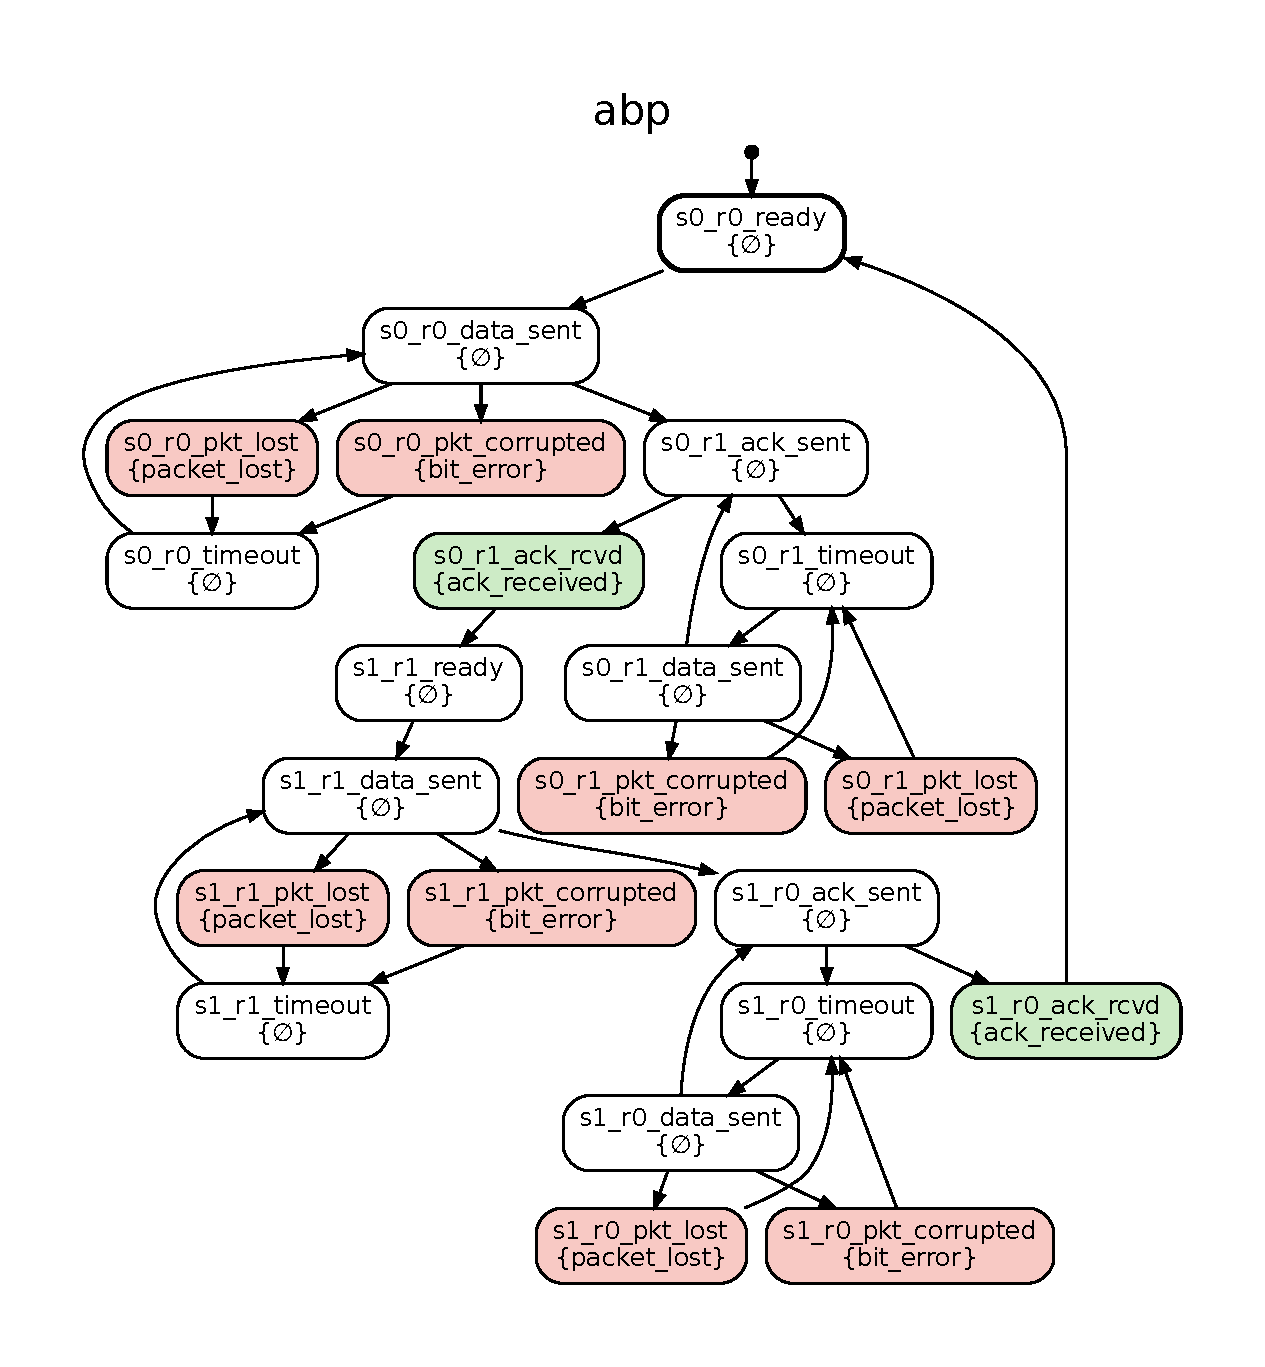
\includegraphics[height=0.5\textheight]{figures/abp.pdf}
\caption{Alternating Bit Protocol: 22 states, 32 transitions. Red: lost or
corrupted packet (entry to the timeout loop). Green: ACK received.}
\label{fig:abp}
\end{figure}

% ---------------------------------------------------------------------
\subsection{Railway Crossing Controller}

\begin{center}\small
\begin{tabularx}{\textwidth}{lll L}
\toprule
\textbf{Kind} & \textbf{Name} & \textbf{Domain / definition} & \textbf{Meaning}\\
\midrule
variable & \code{train} & \{Far, Approaching, InCrossing, Passed\} & train position\\
variable & \code{gate} & \{Open, Lowering, Closed, Raising\} & barrier status\\
variable & \code{ctrl} & \{Idle, ClosingRequested, OpeningRequested\} & controller mode\\
proposition & \code{train_in_crossing} & \code{train = InCrossing} & \\
proposition & \code{gate_is_down} & \code{gate = Closed} & \\
proposition & \code{unsafe_state} & \code{train = InCrossing & gate != Closed} & collision hazard\\
\bottomrule
\end{tabularx}
\end{center}

\textbf{State IDs.} \code{<train>__<gate>__<ctrl>}, initial state
\code{Far__Open__Idle}.

\textbf{Size.} There are $4\cdot4\cdot3=48$ possible combinations. 29 are
reachable, with 80 transitions, and six of the reachable states are unsafe:
\begin{center}\small
\begin{tabular}{p{0.46\textwidth}p{0.46\textwidth}}
\code{InCrossing__Open__Idle} & \code{InCrossing__Open__OpeningRequested}\\
\code{InCrossing__Open__ClosingRequested} & \code{InCrossing__Lowering__OpeningRequested}\\
\code{InCrossing__Lowering__ClosingRequested} & \code{InCrossing__Raising__OpeningRequested}\\
\end{tabular}
\end{center}
The quickest way to reach an unsafe state is the fast-train scenario:
\code{Far__Open__Idle} $\to$ \code{Approaching__Open__Idle} $\to$
\code{InCrossing__Open__ClosingRequested}. The train enters the crossing in the
same step in which the controller gives the closing command, so the gate is
still open.

\begin{figure}[H]
\centering
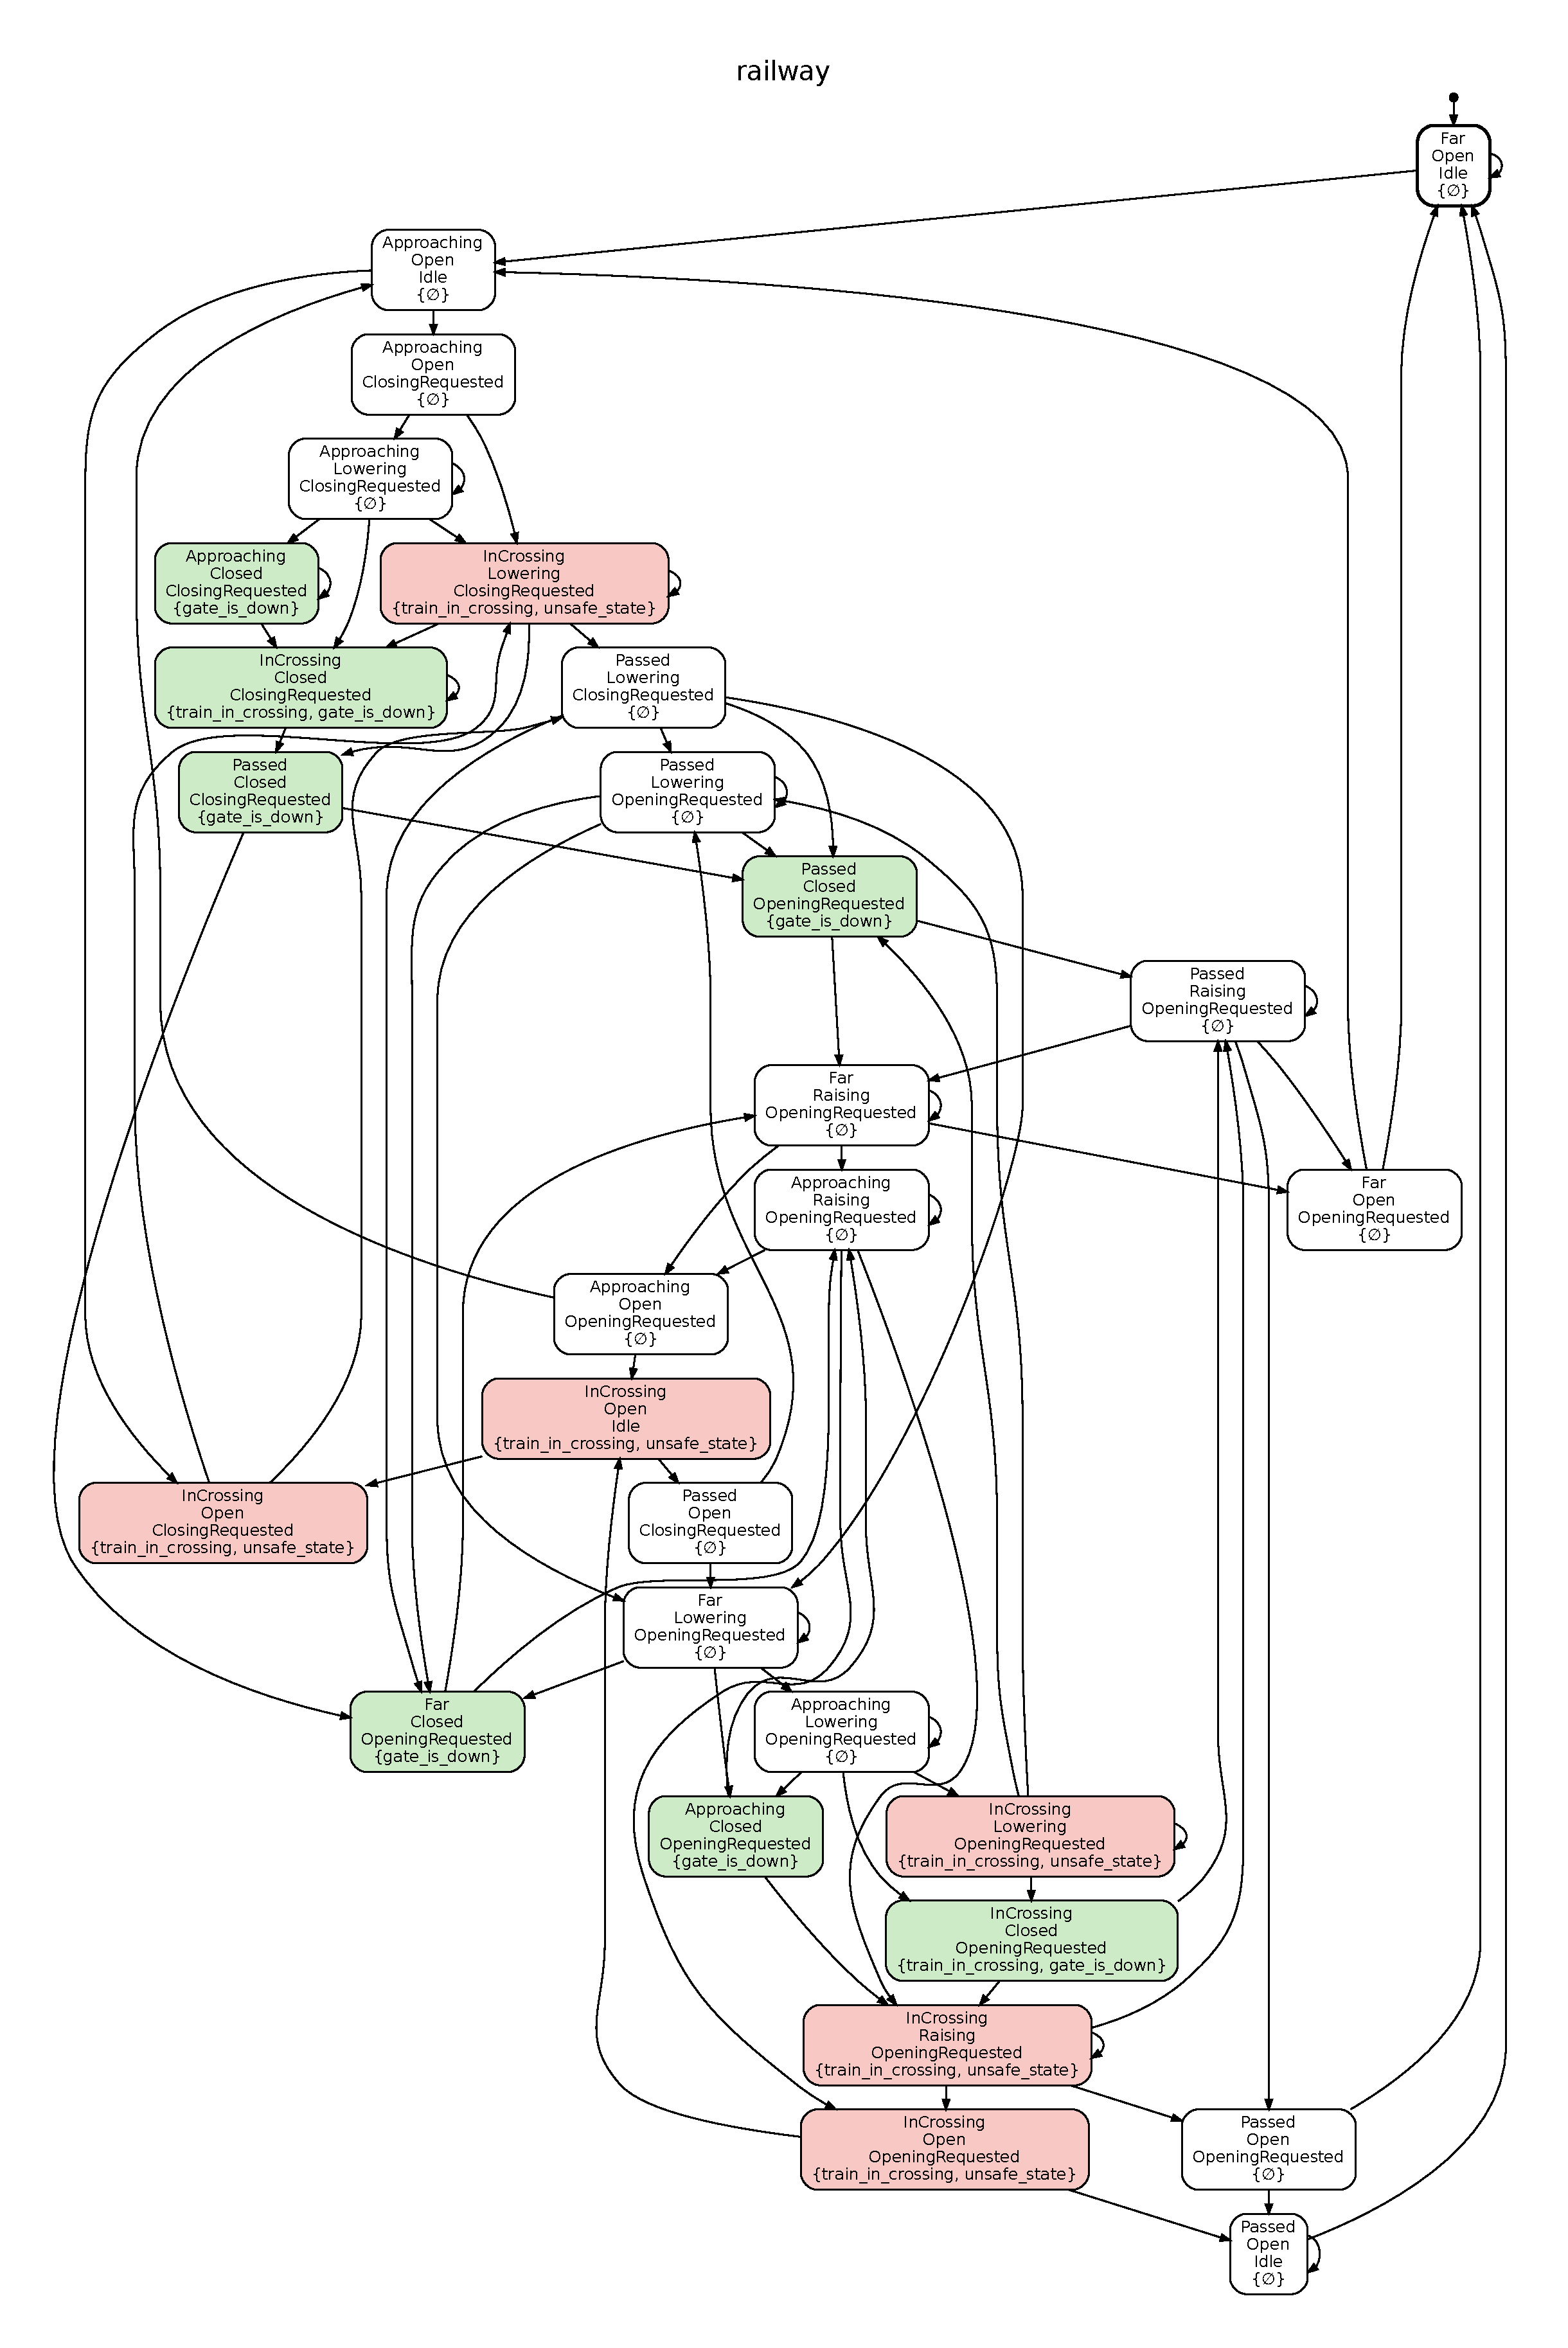
\includegraphics[width=\textwidth,height=0.85\textheight,keepaspectratio]{figures/railway.pdf}
\caption{Railway crossing: 29 states, 80 transitions. Red: \code{unsafe_state}.
Green: gate closed.}
\label{fig:railway}
\end{figure}

% ---------------------------------------------------------------------
\subsection{Three-Floor Elevator Controller}

\begin{center}\small
\begin{tabularx}{\textwidth}{lll L}
\toprule
\textbf{Kind} & \textbf{Name} & \textbf{Domain / definition} & \textbf{Meaning}\\
\midrule
variable & \code{pos} & \{F1, F1\_2, F2, F2\_3, F3\} & floors and intermediate positions\\
variable & \code{dir} & \{Up, Down, Stationary\} & movement direction\\
variable & \code{door} & \{Closed, Opening, Open, Closing\} & door status\\
variable & \code{req} & \{none, F1, F2, F3\} & active destination request\\
variable & \code{stalled} & boolean & emergency stop has occurred\\
input & \code{call}, \code{emergency} & floor call, boolean & environment\\
proposition & \code{moving} & \code{dir != Stationary} & \\
proposition & \code{doors_open} & \code{door = Open} & \\
proposition & \code{stalled} & \code{stalled = TRUE} & \\
\bottomrule
\end{tabularx}
\end{center}

\textbf{State IDs.} \code{<pos>__<dir>__<door>__req_<req>}, with suffix
\code{__STALLED} for stalled states. Examples are
\code{F2_3__Up__Closed__req_F3} and
\code{F1_2__Stationary__Closed__req_F2__STALLED}.

\textbf{Size.} There are $5\cdot3\cdot4\cdot4\cdot2=480$ possible
combinations, but only 43 are reachable, with 58 transitions. They fall into
the following groups:

\begin{center}\small
\begin{tabular}{lr}
\toprule
\textbf{Group of reachable states} & \textbf{Count}\\
\midrule
Idle (one per floor) & 3\\
Request pending: stationary, doors closed (3 floors $\times$ 3 requests) & 9\\
Door cycle Opening / Open / Closing (3 floors) & 9\\
Moving up & 8\\
Moving down & 8\\
Stalled (2 intermediate positions $\times$ 3 requests) & 6\\
\midrule
Total & 43\\
\bottomrule
\end{tabular}
\end{center}

\code{moving} is true in 16 states and \code{doors_open} in 3
(\code{Fk__Stationary__Open__req_Fk}). These two groups do not overlap, so no
reachable state has \code{moving} and \code{doors_open} together. The shortest
way to a stalled state is a call to F2, the cabin starting upwards, reaching
F1\_2 and then an emergency stop:
\code{F1__Stationary__Closed__req_none} $\to$
\code{F1__Stationary__Closed__req_F2} $\to$ \code{F1__Up__Closed__req_F2}
$\to$ \code{F1_2__Up__Closed__req_F2} $\to$
\code{F1_2__Stationary__Closed__req_F2__STALLED}.

\begin{figure}[H]
\centering
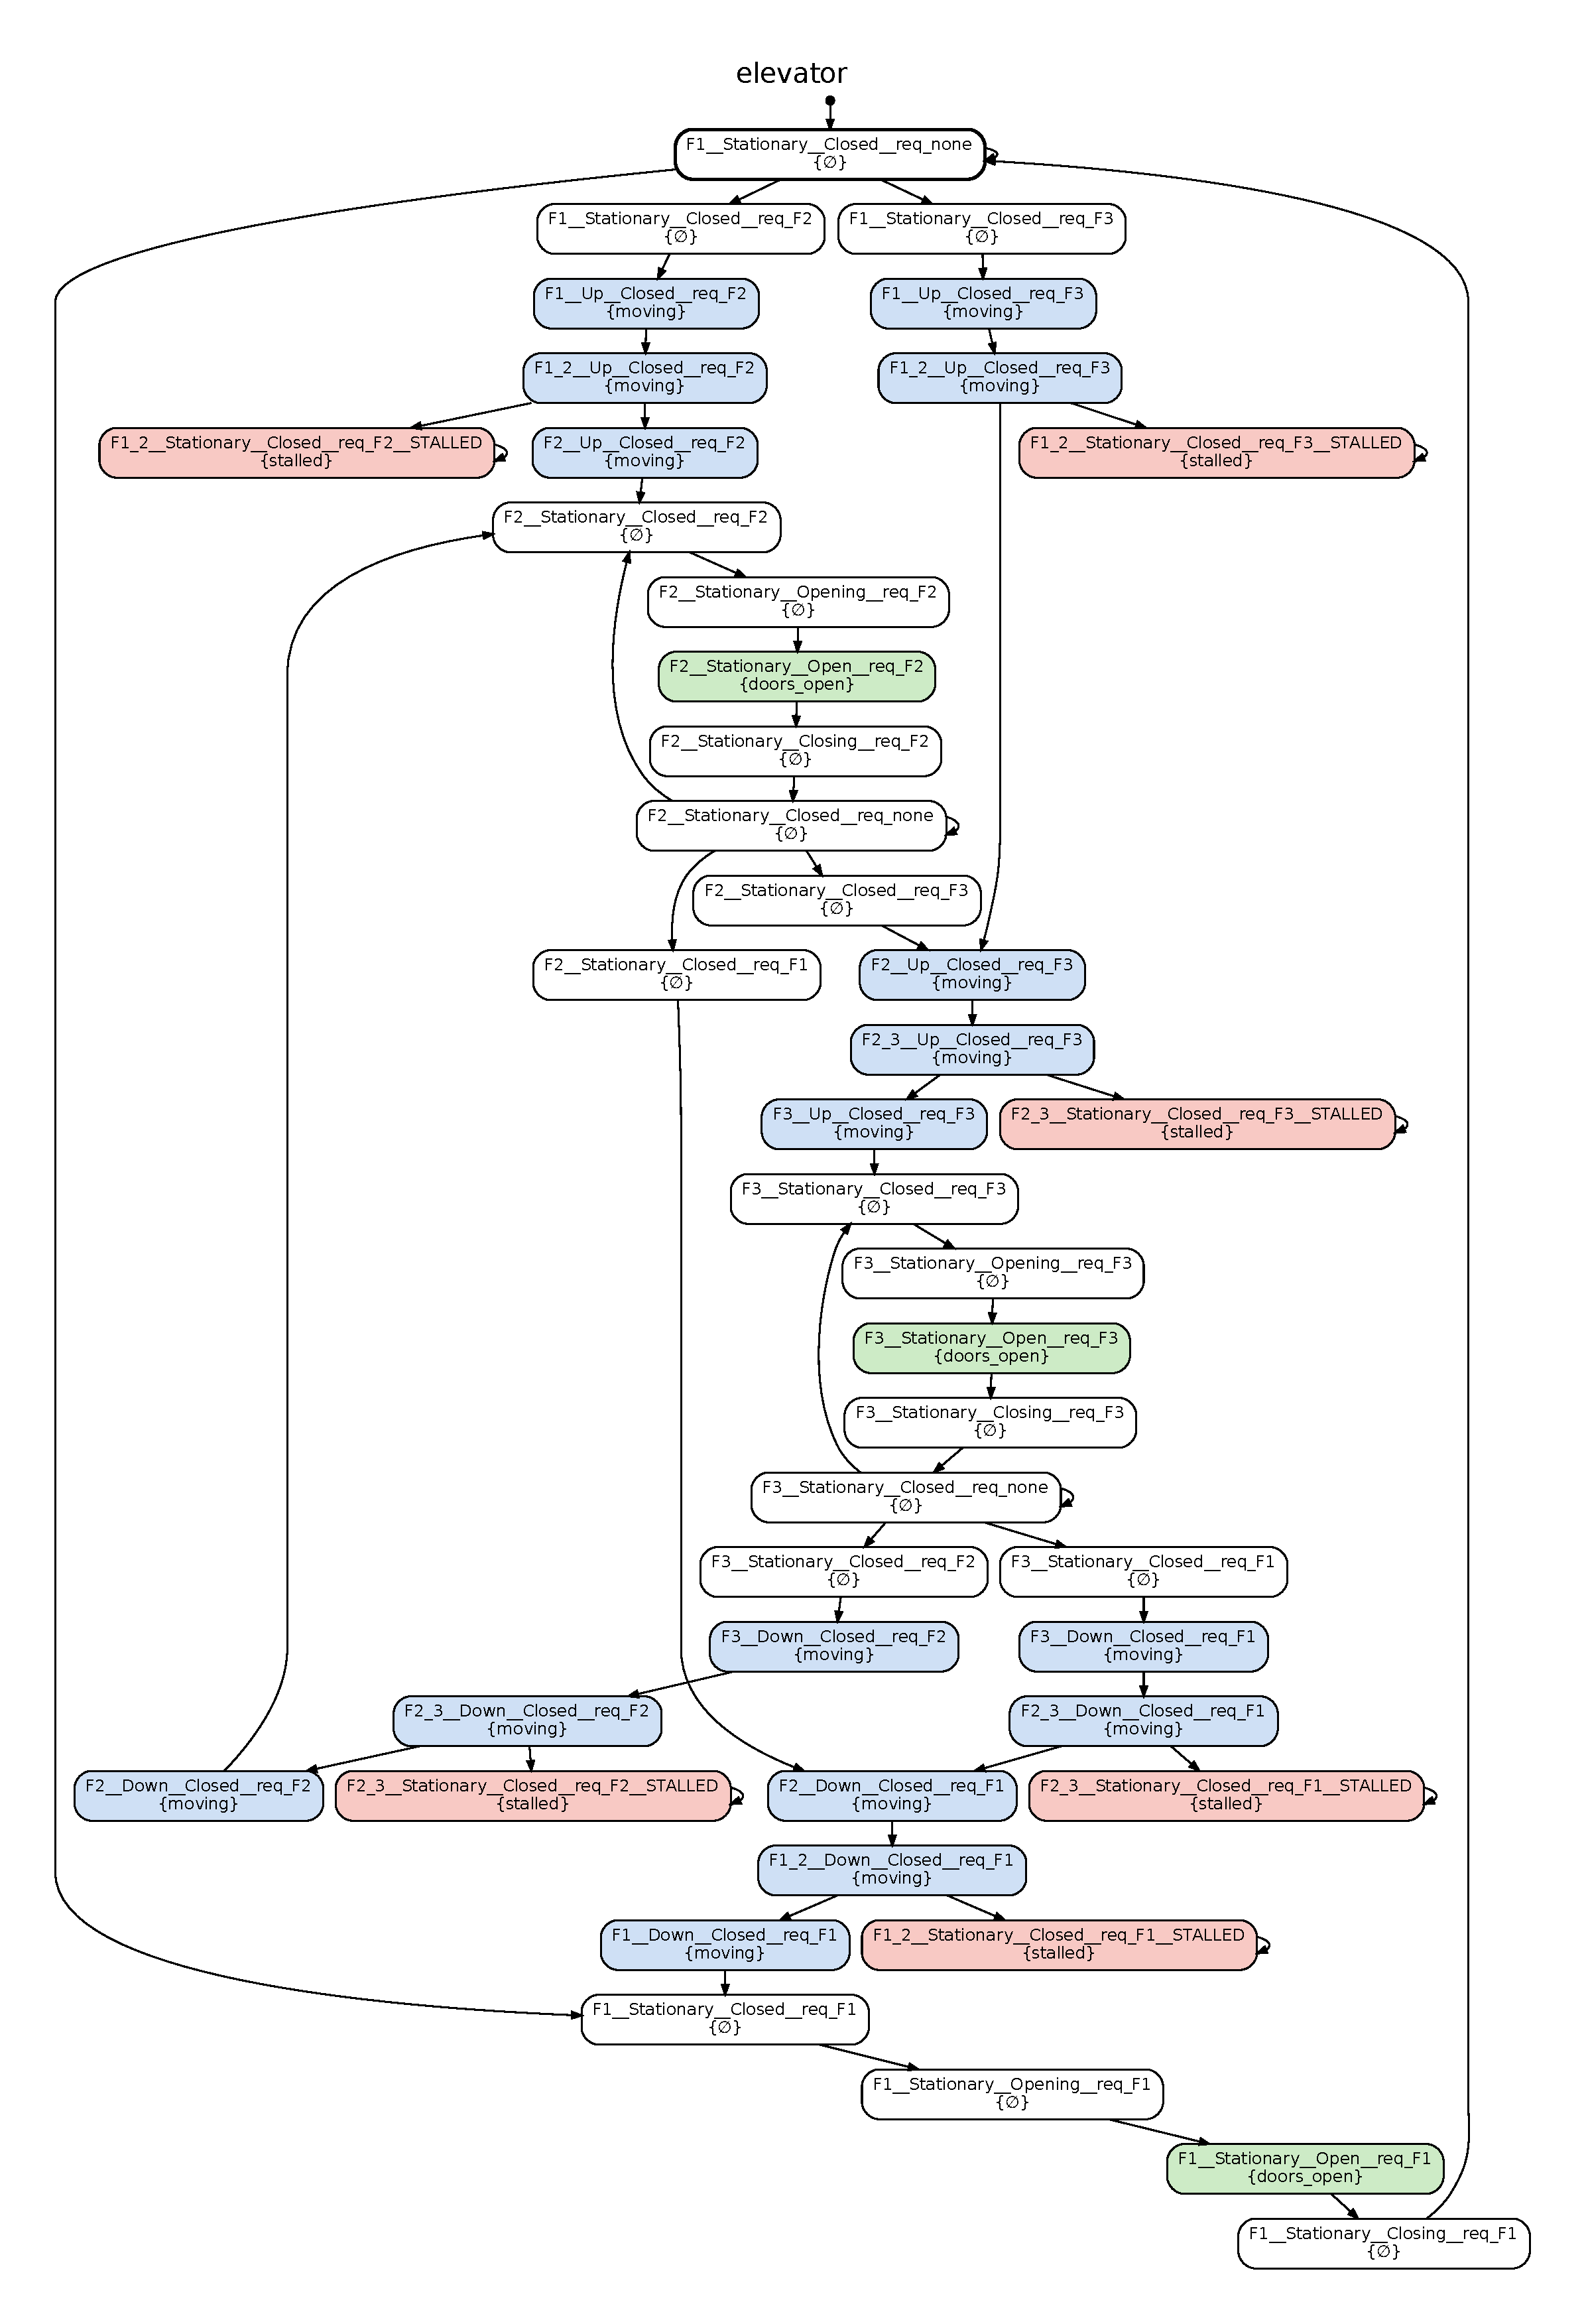
\includegraphics[width=\textwidth,height=0.85\textheight,keepaspectratio]{figures/elevator.pdf}
\caption{Elevator: 43 states, 58 transitions. Blue: \code{moving}. Green:
\code{doors_open}. Red: \code{stalled} (terminal, self-loop).}
\label{fig:elevator}
\end{figure}

% =====================================================================
\section{Implementation Details}
\label{sec:impl}

We wrote \code{my_checker} in Python~3; the code is in
\code{src/checker.py}. It only uses the standard modules \code{json},
\code{sys} and \code{collections}, and we did not use any graph library: the
graph is our own adjacency-list structure. The file \code{my_checker} in the
project root is a short shell script that finds the project folder and runs
\code{python3 src/checker.py "$@"}, so the tool works no matter which
directory it is started from.

\begin{figure}[H]
\centering
\begin{tikzpicture}[
  box/.style={draw, rounded corners, align=center, font=\small,
              minimum height=1.05cm, text width=2.35cm, fill=codebg},
  err/.style={font=\scriptsize\ttfamily, text=red!70!black},
  >={Stealth[length=2mm]}]
\node[box] (a) {\code{parse_args}\\CLI check};
\node[box, right=0.45cm of a] (b) {\code{load_json}\\syntax};
\node[box, right=0.45cm of b] (c) {\code{validate_schema}\\schema};
\node[box, right=0.45cm of c] (d) {\code{validate_semantics}\\6 rules};
\node[box, right=0.45cm of d] (e) {\code{reachable_states}\\BFS};
\draw[->] (a)--(b); \draw[->] (b)--(c); \draw[->] (c)--(d); \draw[->] (d)--(e);
\node[err, below=0.15cm of b] {[SYNTAX ERROR]};
\node[err, below=0.15cm of c] {[SCHEMA ERROR]};
\node[err, below=0.15cm of d] {[SEMANTIC ERROR]};
\node[font=\scriptsize, below=0.15cm of e] {5 lines on stdout};
\node[font=\scriptsize, above=0.1cm of c] {\code{build_nodes}};
\node[font=\scriptsize, above=0.1cm of e] {\code{link_transitions}};
\end{tikzpicture}
\caption{Processing pipeline of \code{my_checker}. Every error stops the
program with a message on standard error and exit code 1. Usage errors exit
with code 2.}
\end{figure}

\subsection{Phase 1: file ingestion and graph construction}

\paragraph{Argument handling.} \code{parse_args} only accepts
\code{--parse <model.json>}. For anything else it prints a usage line to
standard error and exits with code 2.

\paragraph{Syntax.} \code{load_json} opens the file as UTF-8 and parses it
with \code{json.load}. If the file cannot be read or is not valid JSON, we
print a \code{[SYNTAX ERROR]} message with the line and column of the problem.
One detail we had to handle: when the same key appears twice in a JSON object,
Python's parser keeps the last value without any warning. To catch cases like
a state that is declared twice, we pass an \code{object_pairs_hook}
(\code{remember_duplicates}) to the parser, which records every repeated key.
These are reported later as a semantic error.

\paragraph{Schema.} \code{validate_schema} checks that the file follows the
common schema exactly:
\begin{itemize}
  \item the top level is an object with exactly the keys
    \code{atomic_propositions}, \code{initial_states} and \code{states}
    (\code{check_keys} reports both missing and extra keys);
  \item \code{atomic_propositions} and \code{initial_states} are lists of
    strings (\code{check_string_list});
  \item \code{states} is an object, each state is an object with exactly the
    keys \code{labels} and \code{transitions}, and both of these are lists of
    strings.
\end{itemize}
If any of these fails we print a \code{[SCHEMA ERROR]} that names the key and
the JSON type that was found instead.

\paragraph{Graph data structure.} We store the graph as an adjacency list.
Each declared state becomes a \code{Node} object with the three things the
assignment asks for:

\begin{lstlisting}[style=py]
class Node:
    def __init__(self, state_id, labels):
        self.id = state_id          # (a) unique identifier string
        self.labels = set(labels)   # (b) set of active atomic propositions
        self.successors = []        # (c) ordered list of references to target Node objects

class KripkeGraph:
    def __init__(self):
        self.nodes = {}             # state id -> Node   (adjacency list)
        self.initial = []           # Node references of the initial states
\end{lstlisting}

We build the graph in two steps. First, \code{build_nodes} creates a
\code{Node} for every key in \code{states}. Then, after the semantic checks
have passed, \code{link_transitions} replaces each target name with a
reference to the target \code{Node}, keeping the order of the
\code{transitions} list. We link only after validation so that a reference can
never point to a state that does not exist. During the search we can then
follow the references directly instead of looking up names.

\subsection{Phase 2: structural safety and semantic verification}

\code{validate_semantics} checks the six rules from the assignment. As soon as
one of them is violated, the program prints
\code{[SEMANTIC ERROR]: <description>} and exits with code 1.

\begin{center}\small
\begin{tabularx}{\textwidth}{lL}
\toprule
\textbf{Rule} & \textbf{Check performed}\\
\midrule
1.\ Dangling transitions & every transition target is a declared state\\
2.\ Invalid labels & every label is a declared atomic proposition\\
3.\ Transition totality & every state has at least one outgoing transition (deadlocks must use self-loops)\\
4.\ Invalid initial states & \code{initial_states} is non-empty and every entry is a declared state\\
5.\ Duplicate declarations & no repeated entry in \code{atomic_propositions}, \code{initial_states}, or any state's \code{labels} or \code{transitions}; no repeated key in any JSON object (from \code{remember_duplicates})\\
6.\ Empty state space & \code{states} contains at least one state\\
\bottomrule
\end{tabularx}
\end{center}

The table uses the numbering of the assignment, but the code checks the rules
in a different order. It starts with the model as a whole (rule~6, then
rule~5 for the global lists, then rule~4) and only then goes through the
states one by one, checking rule~5 for the state's own lists and then
rules~2, 3 and~1. We chose this order so that, when a model has several
problems, the most basic one is reported first. For example, an empty model
is reported as empty and not as having an invalid initial state. Duplicates
are found in a single pass using a set (\code{find_duplicate}). Unreachable
states are not checked here, because they are not errors.

\subsection{Phase 3: reachability exploration and diagnostics}

\code{reachable_states} runs a breadth-first search that starts only from the
initial states:

\begin{lstlisting}[style=py]
def reachable_states(graph):
    visited = set()
    queue = deque()
    for node in graph.initial:              # start strictly from initial states
        visited.add(node.id)
        queue.append(node)
    while queue:
        node = queue.popleft()
        for succ in node.successors:        # follow Node references
            if succ.id not in visited:
                visited.add(succ.id)
                queue.append(succ)
    return visited
\end{lstlisting}

Each node enters the queue at most once and each edge is looked at once, so
the search takes $O(|S|+|R|)$ time and $O(|S|)$ memory. The number of
unreachable states is $|S| - |\textit{visited}|$. We print it as a diagnostic
and the program continues normally. The transition count is the total length
of all successor lists (\code{KripkeGraph.transition_count}). Since duplicate
transitions are already rejected in Phase~2, this is the number of distinct
directed edges, including self-loops.

\paragraph{Output and exit codes.} When the model is valid, the program prints
the five required lines to standard output and exits with 0. Nothing else is
written to standard output. Every error goes to standard error and the
program exits with a non-zero code.

\subsection{Supporting scripts}

Besides the checker itself, the project contains a few helper scripts:
\begin{itemize}
  \item \code{scripts/gen_<system>.py}: one generator per system. It contains
    the rules and labels of the system, explores the states with BFS from the
    initial state and writes \code{models/<system>.json}.
  \item \code{scripts/draw_model.py} and \code{scripts/report_figures.py}:
    turn a JSON model into a Graphviz drawing and render the state diagrams.
  \item \code{scripts/run_all.sh}: runs \code{my_checker} on every model and
    test file and NuSMV on every \code{.smv} model, and saves the outputs in
    \code{report/outputs/}. The listings in Sections~\ref{sec:test}
    and~\ref{sec:nusmv} are taken directly from there.
  \item \code{scripts/compare_nusmv.py}: reads the list of states printed by
    NuSMV's \code{print_reachable_states -v}, converts each one to the JSON
    naming of the model and compares the two sets of states
    (Section~\ref{sec:nusmv}).
\end{itemize}

% =====================================================================
\section{Testing and Validation}
\label{sec:test}

\subsection{Parser test suite}

We ran \code{my_checker} on the light-switch example, on the five test cases
required by the assignment (marked with $\star$), and on some extra models so
that every syntax, schema and semantic rule is tested at least once. Each
invalid model is the light switch with one mistake added. The outputs in the
table are the real console outputs, saved in \code{report/outputs/checker/}.

{\small
\begin{longtable}{>{\raggedright}p{3.9cm} >{\raggedright}p{2.7cm} >{\raggedright}p{7.2cm} c}
\toprule
\textbf{Test file} & \textbf{Case} & \textbf{Output} & \textbf{Exit}\\
\midrule
\endhead
\code{switch_model.json} & valid example & 2 states, 4 transitions, 2 reachable, 0 unreachable & 0\\
$\star$\,\code{test1_dangling.json} & undeclared transition target & \code{[SEMANTIC ERROR]: State 's_on' references undeclared state 's_ghost'.} & 1\\
$\star$\,\code{test2_bad_label.json} & undeclared label & \code{[SEMANTIC ERROR]: State 's_off' uses undeclared atomic proposition 'is_dark'.} & 1\\
$\star$\,\code{test3_no_transitions.json} & empty transitions & \code{[SEMANTIC ERROR]: State 's_on' has no outgoing transitions (use a self-loop for deadlocks).} & 1\\
$\star$\,\code{test4_bad_initial.json} & undeclared initial state & \code{[SEMANTIC ERROR]: Initial state 's_start' is not declared in 'states'.} & 1\\
$\star$\,\code{test5_unreachable.json} & unreachable state & 3 states, 5 transitions, 2 reachable, \textbf{1 unreachable} & 0\\
\midrule
\code{test6_empty_states.json} & empty \code{states} & \code{[SEMANTIC ERROR]: Model declares no states ('states' is empty).} & 1\\
\code{test7_empty_initial.json} & empty \code{initial_states} & \code{[SEMANTIC ERROR]: 'initial_states' must contain at least one state.} & 1\\
\code{test8_duplicate_prop.json} & duplicate proposition & \code{[SEMANTIC ERROR]: Atomic proposition 'is_lit' is declared more than once.} & 1\\
\code{test9_duplicate_transition.json} & duplicate transition & \code{[SEMANTIC ERROR]: State 's_off' has duplicate transition to 's_on'.} & 1\\
\code{test10_duplicate_state_key.json} & state declared twice & \code{[SEMANTIC ERROR]: Duplicate key 's_on' declared more than once.} & 1\\
\code{test11_duplicate_label.json} & duplicate label & \code{[SEMANTIC ERROR]: State 's_on' has duplicate label 'is_lit'.} & 1\\
\midrule
\code{broken.json} & invalid JSON & \code{[SYNTAX ERROR]: Invalid JSON at line 1, column 36: Illegal trailing comma before end of object} & 1\\
\code{schema_missing_key.json} & missing top-level key & \code{[SCHEMA ERROR]: Top-level object is missing required key(s): initial_states} & 1\\
\code{schema_extra_key.json} & unexpected top-level key & \code{[SCHEMA ERROR]: Top-level object contains unexpected key(s): foo} & 1\\
\code{schema_bad_state_key.json} & unexpected state key & \code{[SCHEMA ERROR]: State 's_off' contains unexpected key(s): color} & 1\\
\code{schema_wrong_type.json} & wrong field type & \code{[SCHEMA ERROR]: 'atomic_propositions' must be an array, got string} & 1\\
\bottomrule
\end{longtable}
}

As required, the first four mandatory cases are rejected with a semantic
error and a non-zero exit code, while the fifth is accepted and reports one
unreachable state. Here are the full outputs for the valid example and for
the unreachable-state case:

\console{outputs/checker/switch_model.txt}{\code{my_checker} on the light-switch example}
\console{outputs/checker/test5_unreachable.txt}{Unreachable-state diagnostics (mandatory case 5). The state \code{s_broken} is declared but cannot be reached from \code{s_off}.}

For comparison, NuSMV also finds 2 reachable states in
\code{tests/switch_model.smv}, the same as \code{my_checker}:

\console{outputs/nusmv/switch_model.txt}{NuSMV on the light-switch example}

\subsection{The five system models}

All five of our JSON models pass validation:

\console{outputs/checker/philosophers.txt}{\code{my_checker} on the Dining Philosophers model}
\console{outputs/checker/peterson.txt}{\code{my_checker} on the Peterson model}
\console{outputs/checker/abp.txt}{\code{my_checker} on the ABP model}
\console{outputs/checker/railway.txt}{\code{my_checker} on the Railway model}
\console{outputs/checker/elevator.txt}{\code{my_checker} on the Elevator model}

Apart from running the checker, we also checked the requirements specific to
each problem on the JSON models:
\begin{itemize}
  \item each model uses exactly the propositions listed in the assignment;
  \item in Philosophers, only \code{s_LLL} has the \code{deadlock} label, and
    it has a self-loop;
  \item in Peterson, no state has both \code{P0_in_CS} and \code{P1_in_CS};
  \item in Railway, \code{unsafe_state} holds exactly in the states where
    \code{train_in_crossing} holds and \code{gate_is_down} does not;
  \item in Elevator, no state has both \code{moving} and \code{doors_open},
    and every stalled state has a self-loop as its only transition.
\end{itemize}
The matching properties of the SMV models are checked with NuSMV in
Section~\ref{sec:nusmv}.

% =====================================================================
\section{NuSMV Comparison}
\label{sec:nusmv}

\subsection{Procedure}

We loaded each \code{.smv} model in NuSMV~2.7.1~\cite{nusmv} in interactive
mode. \code{print_reachable_states} gives the number of reachable states, and
\code{check_invar} and \code{check_ltlspec} check the properties we added to
each model. These properties are not required in Phase~1, but they gave us an
extra way to see whether the SMV models behave as intended. The commands
below are the ones run by \code{scripts/run_all.sh}:

\begin{lstlisting}
$ NuSMV -int models/<system>.smv
NuSMV > go
NuSMV > print_reachable_states
NuSMV > check_invar
NuSMV > check_ltlspec
NuSMV > quit
\end{lstlisting}

NuSMV prints ``reachable states: $r$ out of $d$''. The first number, $r$, is
the number of reachable states. The second, $d$, is the number of all possible
combinations of the \code{VAR} variables, whether they can occur or not.
Input variables (\code{IVAR}) are not part of the state and are not counted.
Our JSON models only contain reachable states, so $r$ is the number to compare
with \code{my_checker}; \code{my_checker} has no equivalent of $d$. The
``system diameter'' printed by NuSMV is the number of BFS layers needed to
reach every reachable state.

Two state sets can have the same size and still be different, so matching
counts alone did not fully convince us. We therefore also compared the sets
themselves. \code{scripts/compare_nusmv.py} takes the complete list of states
printed by \code{print_reachable_states -v}, converts each state to its JSON
name using the mappings given below, and compares the result with the states
in the JSON file.

\console{outputs/nusmv/comparison.txt}{Exact comparison of NuSMV's reachable states with the JSON states\label{lst:cmp}}

\subsection{Results}

\begin{table}[H]
\centering\small
\caption{Reachable-state comparison between \code{my_checker} (JSON) and NuSMV (SMV).}
\label{tab:compare}
\begin{tabular}{lrrrrc}
\toprule
\textbf{System} & \textbf{JSON} & \textbf{my\_checker} & \textbf{NuSMV} & \textbf{NuSMV} & \textbf{Match}\\
 & \textbf{states} & \textbf{reachable} & \textbf{reachable} & \textbf{domain} & \\
\midrule
Dining Philosophers & 14 & 14 & 14 & 27  & \checkmark\\
Peterson            & 20 & 20 & 20 & 32  & \checkmark\\
Alternating Bit     & 22 & 22 & 22 & 28  & \checkmark\\
Railway Crossing    & 29 & 29 & 29 & 48  & \checkmark\\
Elevator            & 43 & 43 & 43 & 480 & \checkmark\\
\bottomrule
\end{tabular}
\end{table}

The reachable-state counts are the same for all five systems. The only
number that differs is NuSMV's $d$, which is larger because it also counts
combinations of values that can never occur. Section~\ref{sec:statespace}
explains, for each system, which combinations these are and why they cannot
be reached.

\subsection{Dining Philosophers}

\textbf{Correspondence.} The SMV state $(p_0,p_1,p_2)$ corresponds to the
JSON state \code{s_XYZ}, where thinking, holding\_left and eating are written
as T, L and E. This SMV model uses an explicit \code{TRANS} relation. Each of
its cases moves one philosopher and leaves the other two unchanged, and a last
case adds the self-loop in the deadlock state. Fork availability is computed
with \code{DEFINE}s, the same way the JSON generator derives it.

\console{outputs/nusmv/philosophers.txt}{NuSMV on \code{models/philosophers.smv}}

\textbf{Discussion.} Both models have 14 reachable states out of 27
combinations; the other 13 are the fork conflicts described in
Section~\ref{sec:statespace}. All four LTL properties hold: two philosophers
never eat at the same time, and once the system is in \code{deadlock} it stays
there (\code{G (deadlock -> X deadlock)}), which shows that the self-loop is
also present in the SMV model. The diameter of 4 means there are four BFS
layers, i.e.\ every state can be reached from \code{s_TTT} in at most three
steps. \code{s_LLL}, for example, is reached after three philosophers each
pick up their left fork.

\subsection{Peterson's Mutual Exclusion}

\textbf{Correspondence.} The SMV state $(pc_0,pc_1,turn)$ corresponds to the
JSON state \code{<pc0>__<pc1>__t<turn>}. The scheduler \code{proc} is an
\code{IVAR}, so it adds transitions but no states. The flags and the other
propositions are \code{DEFINE}s with the same conditions as the JSON labels.

\console{outputs/nusmv/peterson.txt}{NuSMV on \code{models/peterson.smv}}

\textbf{Discussion.} Both models have 20 reachable states out of 32
combinations. Among the 12 that cannot be reached are the states where both
processes are in \code{critical}. NuSMV reports that
\code{G !(P0_in_CS & P1_in_CS)} holds, so mutual exclusion is also satisfied
in the SMV model.

\subsection{Alternating Bit Protocol}

\textbf{Correspondence.} The SMV state $(s\_bit, r\_bit, phase)$ corresponds
to the JSON state \code{s<s_bit>_r<r_bit>_<phase>}. The channel is an
\code{IVAR}.

\console{outputs/nusmv/abp.txt}{NuSMV on \code{models/abp.smv}}

\textbf{Discussion.} Both models have 22 reachable states out of 28
combinations. The 6 missing ones are excluded by the two properties of the
bits explained in Section~\ref{sec:statespace}. The checked properties show
that at most one of the three outcome propositions is true at a time, and
that a lost or corrupted packet always leads to \code{timeout} in the next
step.

\subsection{Railway Crossing Controller}

\textbf{Correspondence.} The SMV state $(train, gate, ctrl)$ corresponds to
the JSON state \code{<train>__<gate>__<ctrl>}. All three \code{next}
assignments use the values of the current state, which is how the synchronous
product is expressed in SMV.

\console{outputs/nusmv/railway.txt}{NuSMV on \code{models/railway.smv}}

\textbf{Discussion.} Both models have 29 reachable states out of 48
combinations. As we expected, the safety invariant \code{!unsafe_state} does
\emph{not} hold. The counterexample NuSMV gives, (Far, Open, Idle) $\to$
(Approaching, Open, Idle) $\to$ (InCrossing, Open, ClosingRequested), is the
same fast-train path we found in Section~\ref{sec:statespace}. This shows that
the controller as specified cannot prevent the fast-train hazard, which is the
situation the problem asks us to find.

\subsection{Three-Floor Elevator Controller}

\textbf{Correspondence.} The SMV state $(pos, dir, door, req, stalled)$
corresponds to the JSON state \code{<pos>__<dir>__<door>__req_<req>}, with
\code{__STALLED} added at the end when \code{stalled} is true. \code{call} and
\code{emergency} are \code{IVAR}s.

\console{outputs/nusmv/elevator.txt}{NuSMV on \code{models/elevator.smv}}

\textbf{Discussion.} Both models have 43 reachable states out of 480
combinations, and all checked properties hold. The first invariant,
\code{!(moving & doors_open)}, is the requirement from the assignment. The
second, \code{moving -> door = Closed}, is a little stronger: the cabin only
moves when the doors are fully closed. The third invariant and the LTL
property show that after an emergency stop the cabin is between floors, not
moving and with its doors locked, and that it stays stalled. The diameter of
16 is large because serving a request is a long and almost fixed sequence of
steps.

\subsection{Conclusion}

For all five systems, the JSON model and the separately written NuSMV model
describe the same transition system. \code{my_checker} and NuSMV find the same
number of reachable states, and the reachable states themselves are also the
same (Listing~\ref{lst:cmp}). The only remaining difference in NuSMV's output
is the total number of combinations, and this is explained by the value
combinations that the system rules never allow.

% =====================================================================
\clearpage
\begin{thebibliography}{9}
\addcontentsline{toc}{section}{References}

\bibitem{assignment}
A.~E. Uğur, N.~F. Altunel and M.~T. Sandıkkaya,
\emph{BLG~345E Logic and Computability -- Term Project Phase~1: Structural
Modeling, Parsing and Oracle Validation},
project assignment document, Istanbul Technical University, Faculty of Computer
and Informatics Engineering, Fall 2026.


\bibitem{slides}
M.~T. Sandıkkaya,
\emph{Logic \& Computability -- Week~5 lecture handout: Proving and
Verification with Model Checking} (Automated Reasoning, Model Checking,
Program Verification),
BLG~345E lecture notes, Istanbul Technical University, Computer Engineering
Department, Fall 2026/27.


\bibitem{nusmv}
R.~Cavada, A.~Cimatti, C.~A. Jochim, G.~Keighren, E.~Olivetti, M.~Pistore,
M.~Roveri and A.~Tchaltsev,
\emph{NuSMV 2.6 User Manual},
Fondazione Bruno Kessler (FBK-irst), Trento, Italy.
Available at \url{https://nusmv.fbk.eu}.

\end{thebibliography}

\end{document}
